\documentclass[
  bibliography=totoc,     % Literatur im Inhaltsverzeichnis
  captions=tableheading,  % Tabellenüberschriften
  titlepage=firstiscover, % Titelseite ist Deckblatt
]{scrartcl}

% Paket float verbessern
\usepackage{scrhack}

% Warnung, falls nochmal kompiliert werden muss
\usepackage[aux]{rerunfilecheck}

% unverzichtbare Mathe-Befehle
\usepackage{amsmath}
% viele Mathe-Symbole
\usepackage{amssymb}
% Erweiterungen für amsmath
\usepackage{mathtools}

% Fonteinstellungen
\usepackage{fontspec}
\usepackage{microtype}
\DeclareMicrotypeAlias{LibertinusSerif} {Latin Modern Roman}

% Latin Modern Fonts werden automatisch geladen
% Alternativ:
%\setromanfont{Libertinus Serif}
%\setsansfont{Libertinus Sans}
%\setmonofont{Libertinus Mono}
\recalctypearea % Wenn man andere Schriftarten gesetzt hat,
% sollte man das Seiten-Layout neu berechnen lassen

% deutsche Spracheinstellungen
\usepackage{polyglossia}
\setmainlanguage{german}


\usepackage[
  math-style=ISO,    % ┐
  bold-style=ISO,    % │
  sans-style=italic, % │ ISO-Standard folgen
  nabla=upright,     % │
  partial=upright,   % ┘
  warnings-off={           % ┐
    mathtools-colon,       % │ unnötige Warnungen ausschalten
    mathtools-overbracket, % │
  },                       % ┘
]{unicode-math}

% traditionelle Fonts für Mathematik
\setmathfont{Latin Modern Math}
% Alternativ:
%\setmathfont{Libertinus Math}

\setmathfont{XITS Math}[range={scr, bfscr}]
\setmathfont{XITS Math}[range={cal, bfcal}, StylisticSet=1]

% Zahlen und Einheiten
\usepackage[
  locale=DE,                   % deutsche Einstellungen
  separate-uncertainty=true,   % immer Fehler mit \pm
  per-mode=symbol-or-fraction, % / in inline math, fraction in display math
]{siunitx}
\sisetup{math-micro=\text{µ},text-micro=µ}

% chemische Formeln
\usepackage[
  version=4,
  math-greek=default, % ┐ mit unicode-math zusammenarbeiten
  text-greek=default, % ┘
]{mhchem}

% richtige Anführungszeichen
\usepackage[autostyle]{csquotes}

% schöne Brüche im Text
\usepackage{xfrac}

% Standardplatzierung für Floats einstellen
\usepackage{float}
\floatplacement{figure}{htbp}
\floatplacement{table}{htbp}

% Floats innerhalb einer Section halten
\usepackage[
  section, % Floats innerhalb der Section halten
  below,   % unterhalb der Section aber auf der selben Seite ist ok
]{placeins}

% Seite drehen für breite Tabellen: landscape Umgebung
\usepackage{pdflscape}

% Captions schöner machen.
\usepackage[
  labelfont=bf,        % Tabelle x: Abbildung y: ist jetzt fett
  font=small,          % Schrift etwas kleiner als Dokument
  width=0.9\textwidth, % maximale Breite einer Caption schmaler
]{caption}
% subfigure, subtable, subref
\usepackage{subcaption}

% Grafiken können eingebunden werden
\usepackage{graphicx}
% größere Variation von Dateinamen möglich
\usepackage{grffile}

% schöne Tabellen
\usepackage{booktabs}

% Verbesserungen am Schriftbild
\usepackage{microtype}

% Literaturverzeichnis
\usepackage[
  backend=biber,
]{biblatex}
% Quellendatenbank
\addbibresource{lit.bib}
\addbibresource{programme.bib}

% Hyperlinks im Dokument
\usepackage[
  unicode,        % Unicode in PDF-Attributen erlauben
  pdfusetitle,    % Titel, Autoren und Datum als PDF-Attribute
  pdfcreator={},  % ┐ PDF-Attribute säubern
  pdfproducer={}, % ┘
]{hyperref}
% erweiterte Bookmarks im PDF
\usepackage{bookmark}
%wrapping text around pictures
\usepackage{wrapfig}
% Trennung von Wörtern mit Strichen
\usepackage[shortcuts]{extdash}
\usepackage{blindtext}
\usepackage{longtable}
%fix Problem with micro (siunitx using wrong package) in new latex-version
\usepackage{textcomp}
\newcommand{\upd}{\symup{d}}
\usepackage{braket} %Brackets für Erwartungswert und Varianz
\author{%
Julian Hochhaus%
\texorpdfstring{%
  \\%
  \href{mailto:julian.hochhaus@tu-dortmund.de}{julian.hochhaus@tu-dortmund.de}
}{}%
  \texorpdfstring{\and}{, }%
  Niko Salewski %
  \texorpdfstring{%
    \\%
    \href{mailto:niko.salewski@tu-dortmund.de}{niko.salewski@tu-dortmund.de}
  }{}%
}
\publishers{TU Dortmund – Fakultät Physik}


\subject{V27}
\title{Der Zeeman-Effekt}
\date{
  Durchführung: 16.04.18
  \hspace{3em}
  %Abgabe Korrektur: 
}

\begin{document}

\maketitle
\thispagestyle{empty}
\tableofcontents
\newpage

\setcounter{page}{1}
\section{Zielsetzung}
\label{sec:Zielsetzung}

In diesem Versuch wird der Innenwiderstand und die Leerlaufspannung einer Spannungsquelle bestimmt amina koyim.


\section{Theorie}
\label{sec:Theorie}
Brückenschaltungen werden in der Physik verwendet, um über bereits bekannte Bauelemente die
physikalischen Kennwerte eines unbekannten ohmschen Widerstands oder einer Impedanz zu bestimmen.
Mithilfe der beiden Kirchhoffschen Regeln lassen sich Bedingungen zur Bestimmung unbekannter Elemente in
Brückenschaltungen formulieren.
\subsection{Kirchhoff'sche Regel}

\subsubsection{Knotenregel}
Die Knotenregel besagt anschaulich, dass Ströme, die in einen Knotenpunkt
hineinfließen, auch wieder hinausfließen müssen. Im Knoten selbst dürfen also keine Ströme verschwinden,
oder neu entstehen.
\begin{equation}
  \centering
  \label{eqn:knotenregel}
\sum_{k}{I_K}=0
\end{equation}
Etwas mathematischer ausgedrückt heißt das, dass die Summe über alle eingehenden
und alle ausgehenden Strömen gleich Null sein muss.

\subsubsection{Maschenregel}
Eine Masche bezeichnet einen in sich geschlossenen Stromkreis.
Die Maschenregel besagt, dass für eine Masche die Summe aller Einzelspannungen $U_i$
an den einzelnen Bauelementen, wie zum Beispiel Ohmschen Widerständen, Spulen und Kondensatoren,
gleich der angelegten Gesamtspannung $U_0$ sein muss. Äquivalent dazu ist die Formulierung, dass die Summe aller auftretenden Spannungen $U_k$ gleich Null ist.

\begin{equation}
  \label{eqn:maschenregel}
  \centering
U_0=\sum_{i}{U_i} \Rightarrow \sum_{k}{U_k}=0
\end{equation}
 Eine alternative Formulierung erhält man unter Verwendung des Ohmschen Gesetz. Dieses definiert den elektrischen Widerstand $R$
 als Quotienten aus der anliegenden Spannung $U$ zur Stromstärke $I$ des durch den Widerstand fließenden Stroms.
 Stellt man das Ohmsche Gesetz nach $U$ um, ergibt sich der Zusammenhang
\begin{equation}
   \centering
   U=R \cdot I
 \end{equation}
 Somit kann die Maschenregel auch abhängig von Stromstärke und Widerständen formuliert werden:
 \begin{equation}
   U_0=\sum_{i}{I_i \cdot R_i}
\end{equation}


\begin{figure}
  \centering
  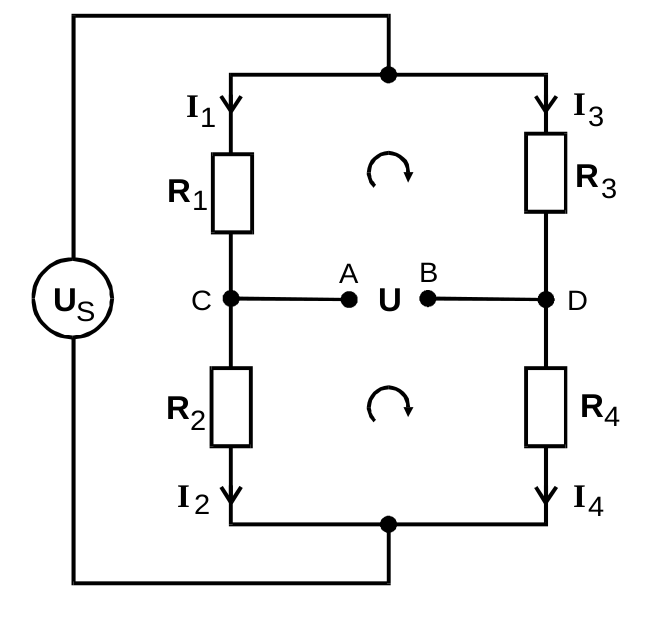
\includegraphics[width=0.7\textwidth]{Bilder/brueckenschaltungallgemein.png}
  \caption{Grundlegender Aufbau einer Brückenschaltung \cite{Anleitung}}
  \label{fig:brückenschaltung}
\end{figure}
In Abbildung \ref{fig:brückenschaltung} ist der schematische Aufbau einer Brückenschaltung dargestellt.
Als Brückenspannung wird hierbei die zwischen den Punkten $A$ und $B$ auftretende Spannung $U_{Br}$ bezeichnet.

Die Brückenschaltung kann man als Parallelschaltung zweier widerstandsbehafteter Leiter verstehen. An diese Parallelschaltung wird dabei die Speisespannung $U_S$ angelegt.
Der Stromfluss teilt sich auf die beiden parallelen Zweige auf. Er fließt damit entweder durch den linken Zweig und somit durch die Widerstände $R_1$ und $R_2$ oder durch den rechten Zweig, also durch $R_3$ und $R_4$.

Mithilfe der Kirchhoffschen Regeln \eqref{eqn:knotenregel} und \eqref{eqn:maschenregel} lässt sich die Brückenspannung $U_{Br}$ abhängig von den verwendeten Widerständen und der angelegten Spannung $U_S$ wie folgt formulieren:
\begin{equation}
  \label{eqn:brückeeingang}
U_{Br}=\frac{R_2R_3-R_1R_4}{(R_3+R_4)(R_1+R_2)}U_S .
\end{equation}
Die Brückenspannung verschwindet, wenn der Zähler gleich Null, also $R_2R_3-R_1R_4=0$ gilt.
Die Brücke wird dann als abgeglichen bezeichnet. Es gilt also:
\begin{equation}
R_2R_3=R_1R_4
\label{eqn:abgleichbedingung}
\end{equation}
Diese sogenannte Abgleichbedingung hängt somit lediglich von den Widerständen ab. Somit lässt sich ein unbekannter Widerstand $R_x$ mittels der abgeglichenen Brücke bestimmen.

Dafür müssen die bekannten Widerstände mit möglichst großer Genauigkeit bekannt sein und mindestens einer der Widerstände muss sich regulieren lassen.

Um eine möglichst genaue Bestimmung des unbekannten Widerstands $R_x$ zu realisieren, muss man die Brückenspannung möglichst genau zu Null abgleichen können.
Dazu wird ein Galvanometer, (Mikro-)Voltmeter oder ein Kathodenstrahloszillograph verwendet.

Da nach Gleichung \eqref{eqn:brückeeingang} ein Zusammenhang zwischen der Speisespannung $U_S$ und der Brückenspannung $U_{Br}$ besteht, wird die Genauigkeit der Messung zudem durch eine möglichst große Speisespannung verbessert.
Schließlich kann anstelle eines ohmschen Widerstands auch ein komplexer Widerstand mittels der abgeglichenen Brücke bestimmt werden. Hierfür muss man allerdings beachten, dass dieser sich aus einen Wirk-und einen Blindwiderstand zusammensetzt.

\subsection{Realisierung komplexer Widerstände von Induktivitäten und Kondensatoren}
\label{sec:komplexewiderstände}
Fließt Strom durch einen Kondensator, so baut sich in diesem ein elektrisches Feld auf. Ähnlich verhält es sich bei Spulen. Hier baut sich bei fließendem Strom ein magnetisches Feld auf.
Einer Spannungsquelle wird also durch angeschlossene Kondensatoren oder Spulen Energie entzogen und im elektrischen bzw. magnetischen Feld gespeichert. Diese wird allerdings nicht umgewandelt in eine andere Energie (z.B. thermische oder mechanische) sondern kann nach einer Umkehrung der Spannungsrichtung zur Quelle zurückgeführt werden.
Daher werden sogenannte Impedanzen (Wechselstromwiderstände) zur Beschreibung von Spulen und Kondensatoren verwendet:
\begin{equation}
\Theta= X+iY
\end{equation}
$X$ ist hierbei der Wirkwiderstand und $Y$ die Reaktanz (Blindwiderstand).
Bei Spulen und Kondensatoren treten zudem Wärmeverluste, zum Beispiel zwischen den Kondensatorplatten
oder in den Drähten auf.

Zur Realisierung solcher sogenannter dielektrischen Verluste
ergänzt man daher das Ersatzschaltbild durch gedachte ohmsche Widerstände $R_x$.
Brückenschaltungen mit komplexen Widerständen müssen somit im Gegensatz zu Schaltungen, welche lediglich ohmsche Widerstände enthalten, mit Wechselstrom betrieben werden, sodass das magnetische bzw. elektrische Feld sich periodisch auf- und auch wieder abbauen kann.

Somit müssen wiederum die Abgleichbedingungen für den Fall, dass Kondensatoren und Spulen in der Brückenschaltung verwendet werden, sowohl Phase, als auch den Wirkwiderstand berücksichtigen.
Im Folgenden soll im Einzelnen auf die fünf verschiedenen Brückenschaltungen eingegangen werden.

\subsection{Wheatstonesche Brückenschaltung}
\begin{figure}
  \centering
  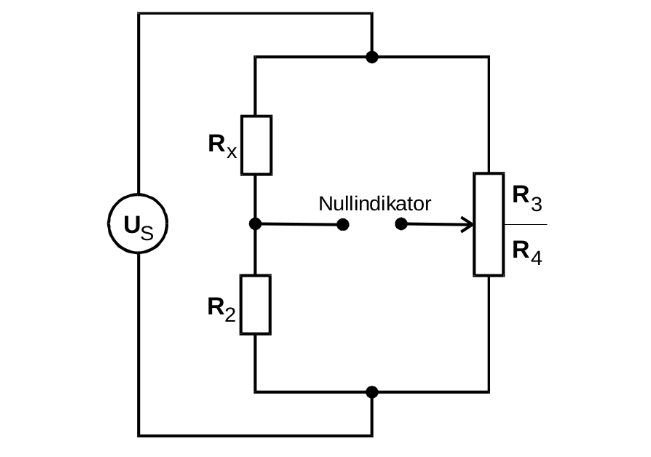
\includegraphics[width=0.9\textwidth]{Bilder/Wheatstone_bruecke.png}
  \caption{Wheatstonesche Brückenschaltung zur Bestimmung eines unbekannten Widerstands \cite{Anleitung}}
  \label{fig:wheatstonebrücke}
\end{figure}

In Schaltbild \ref{fig:wheatstonebrücke} ist die Wheatstonesche Brücke abgebildet. Diese enthält lediglich Ohmsche Widerstände. Daher kann sie sowohl mit Wechselstrom als auch mit Gleichstrom betrieben werden.
Der zu bestimmende Widerstand $R_x$ lässt sich nach \eqref{eqn:abgleichbedingung} über die anderen Widerstände wie folgt bestimmen:
\begin{equation}
  \centering
  R_x=R_2 \cdot \frac{R_3}{R_4};
\label{eqn:widerstand}
\end{equation}
Aus \eqref{eqn:widerstand} ergibt sich, dass die konkreten Werte von $R_3$ und $R_4$ nicht bekannt sein müssen, um $R_x$ zu ermitteln. Es reicht vollkommen, ihr Verhältnis zu kennen.
Daher können $R_3$ und $R_4$ mittels eines Potentiometers realisiert werden.

\subsection{Kapazitätsmessbrücke}
\begin{figure}
  \centering
  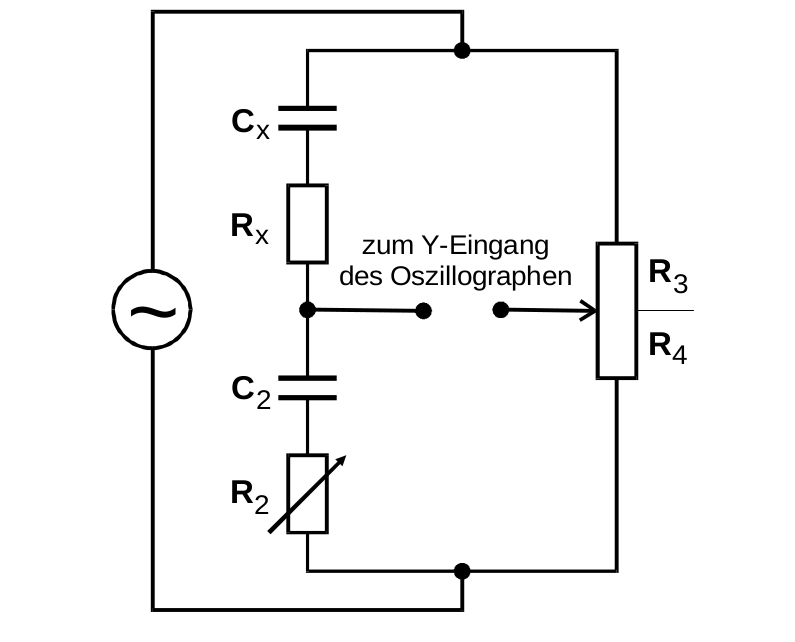
\includegraphics[width=0.7\textwidth]{Bilder/kapazitaetmessbruecke.png}
  \caption{Brückenschaltung zur Bestimmung eines unbekannten Kondensators \cite{Anleitung}}
  \label{fig:kapazitätsmessbrücke}
\end{figure}
Bei der Kapazitätsmessbrücke abgebildet in \ref{fig:kapazitätsmessbrücke} wird ein Kondensator in die Brückenschaltung eingebaut.
Wie bereits in \ref{sec:komplexewiderstände} erklärt, muss daher sowohl die Phase, als auch der Wirkwiderstand abgeglichen werden.
$R_x$ steht hierbei stellvertretend für die Wärmeverluste im Kondensator. Zum Abgleich des komplexen kapazitiven Widerstands wird also eine Ersatzschaltung verwendet.
Hierzu wird ein bekannter Kondensator $C_2$ in Reihe geschaltet zu einem regulierbaren ohmschen Widerstand $R_2$.
$R_2$ ist hierbei regulierbar, um die in der Kapazität entstehende Phasenverschiebung zu kompensieren. Für den $R_2-C_2$-Zweig wird hierbei angenommen, dass $R_{Wirk}=R_2$ gilt, also der Kondensator $C_2$ verlustfrei ist. Dies ist, wie sich auch anhand von $R_x$ nahezu 0 zeigt, realisierbar.
Wenn der unbekannte Kondensator als verlustfrei angenommen werden kann, kann auf den regelbaren Widerstand $R_2$ verzichtet werden.
Dies würde sich auch in der Messung zeigen. Wenn $R_2$ auf $0 \si{\ohm}$ gestellt werden kann und sich die Brückenspannnung trotzdem zu Null abgleichen lässt, kann man den Kondensator als verlustfrei annehmen.
Die Abgleichbedingungen ergeben sich somit zu
\begin{equation}
\centering
\label{eqn:kapwiderstand}
R_x=\frac{R_2R_3}{R_4}
\end{equation}
und
\begin{equation}
\centering
\label{eqn:kapazitaet}
C_x=\frac{C_2R_4}{R_3}
\end{equation}
Aus den Abgleichbedingungen ist ersichtlich, dass das Verhältnis von $R_3$ zu $R_4$ mit \eqref{eqn:kapazitaet} unabhängig von $R_x$ formuliert werden kann.
Die Notwendigkeit der zweiten Abgleichbedingung und damit das Hinzufügen eines ohmschen Widerstands $R_2$ ergibt sich somit nur, wenn $R_x$ ungleich 0 ist.

\subsection{Induktivitätsmessbrücke}

\begin{figure}
  \centering
  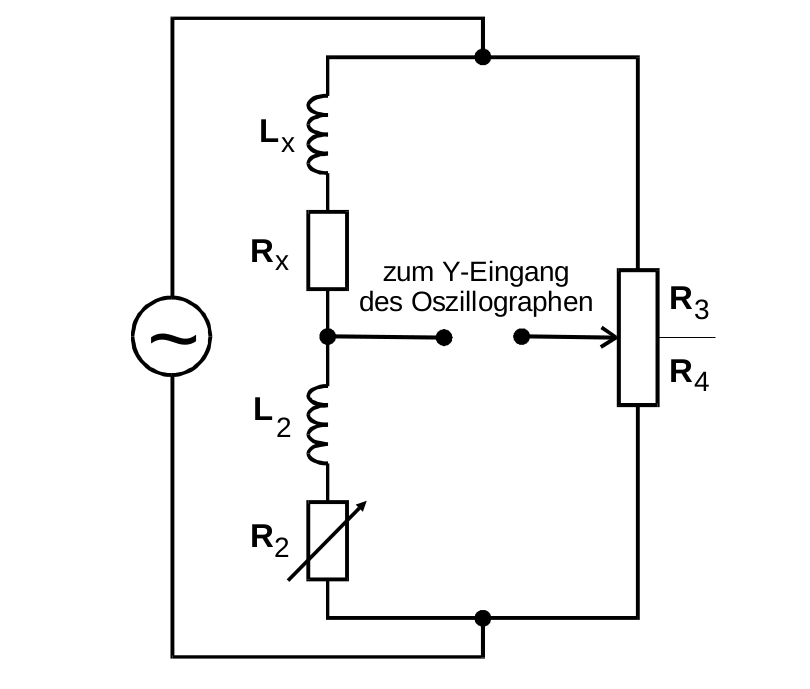
\includegraphics[width=0.9\textwidth]{Bilder/Messbruecke_Spule_mit_R.png}
  \caption{Brückenschaltung zur Bestimmung der Induktivität einer Spule  \cite{Anleitung}}
  \label{fig:induktivitätsmessbrücke}
\end{figure}
In Schaltbild \ref{fig:induktivitätsmessbrücke} ist eine Brückenschaltung zur Messung eines induktiven Widerstands dargestellt.
Es müssen also erneut komplexe Widerstände betrachtet werden. Der prinzipielle Aufbau zur Messung einer realen Spule stellt sich also sehr ähnlich wie die Brückenschaltung zur Bestimmung eines Kondensators dar.
Es müssen lediglich die Kondensatoren $C_i$ an entsprechender Stelle durch Spulen $L_i$ ersetzt werden.
Die Abgleichbedingungen ergeben sich somit zu:
\begin{equation}
\centering
\label{eqn:indukwiderstand}
R_x=\frac{R_2R_3}{R_4}
\end{equation}
und
\begin{equation}
\centering
\label{eqn:induktivität}
L_x=\frac{L_2R_3}{R_4}
\end{equation}
Die bei der Kapazitätsmessbrücke leicht zu realisierende Forderung, dass der Wirkwiderstand im linken unteren Zweigabschnitt gleich dem Widerstand $R_2$ ist,
lässt sich bei Induktivitäten besonders für niedrige Frequenzen nur schwerlich realisieren.
Es lassen sich daher genauere Ergebnisse erzielen, wenn anstelle der Induktivität $L_2$ eine Ersatzschaltung mit einer Kapazität, die sogenannte Maxwell-Brücke, verwendet wird.

\subsection{Maxwell-Brücke}
\begin{figure}
  \centering
  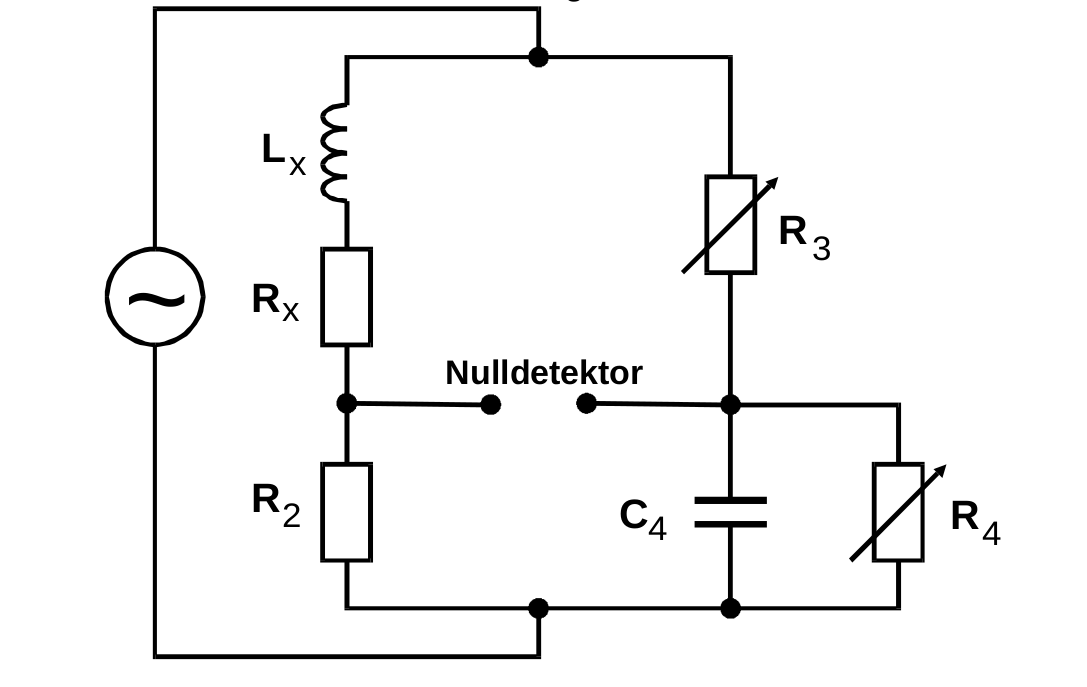
\includegraphics[width=0.9\textwidth]{Bilder/maxwell_bruecke.png}
  \caption{Maxwell-Brücke zur Bestimmung einer Induktivität \cite{Anleitung}}
  \label{fig:maxwellbrücke}
\end{figure}
In der in Abbildung \ref{fig:maxwellbrücke} werden erneut Induktivitäten vermessen.
Wie bereits erwähnt, erzielt man im Gegensatz zur Induktivitätsmessbrücke
mit einer Induktivität $L_2$ hier mit einer eingebauten Kapazität $C_2$ aufgrund der deutlich geringeren Wärmeverluste eine höhere Genauigkeit der messung.
Für die Abgleichbedingungen erhält man, indem man erneut die Kirchhoffschen Regeln nach \eqref{eqn:maschenregel} und \eqref{eqn:knotenregel} verwendet, zu:
\begin{equation}
\label{eqn:maxwellr}
\centering
R_x=\frac{R_2R_3}{R_4}
\end{equation}
und
\begin{equation}
\centering
\label{eqn:maxwellinduktivität}
L_x=R_2R_3C_4
\end{equation}
\subsection{Wien-Robinson-Brücke}
\begin{figure}
  \centering
  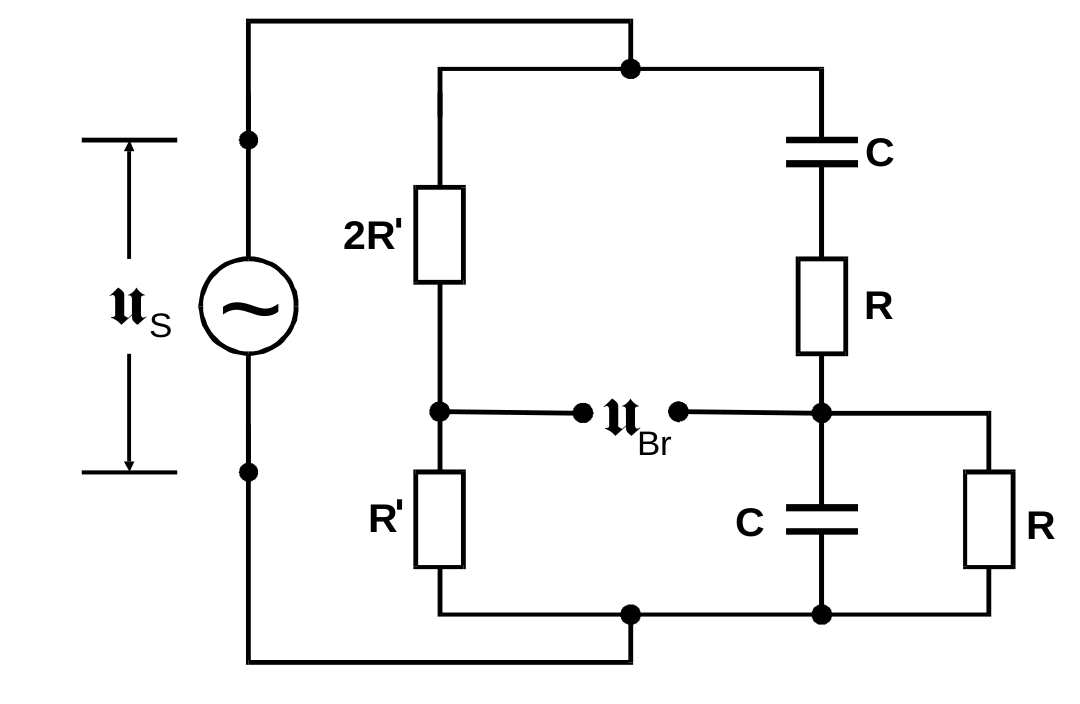
\includegraphics[width=0.9\textwidth]{Bilder/wien_robinson_bruecke.png}
  \caption{Wien-Robinson-Brücke zur Klirrfaktor-Bestimmung \cite{Anleitung}}
  \label{fig:wienrobinsonbrücke}
\end{figure}

In der letzten betrachteten Brückenschaltung sind im Gegensatz zu den vorherigen Brückenschaltungen keine Abgleichelemente enthalten.
Bei den zuvor betrachteten Brückenschaltungen sollte sich prinzipiell also die Abgleichbedingung immer unabhängig von der Frequenz $\omega$ der Speisespannung $U_S$ erfüllen lassen. Dies stimmt allerdings nur eingeschränkt. Für große Frequenzen $\omega$ werden sich allerdings störende Streueffekte zeigen und für kleine Frequenzen dauert es etwas, bis sich ein stationärer Fall einstellt.

Die Wien-Robinson-Brücke dient nun als elektronischer Filter, das heißt, im Gegensatz zu den bisherigen Schaltungen wird die Wien-Robinson-Brücke sich nur bei einer bestimmten Frequenz $\omega=\omega_0$ abgleichen lassen.

Die Ableichbedingung ergibt sich somit über die Frequenz.

Der Quotient aus Speise-und Brückenspannung ergibt sich unter der Verwendung komplexer Widerstände und Kapazitäten zu:

\begin{equation}
\label{eqn:wienquotient}
\left|\frac{U_{Br}}{U_s}\right|^2= \frac{(\omega^2R^2C^2-1)^2}{9 \cdot ((1-\omega^2R^2C^2)^2+9\omega^2R^2C^2)}
\end{equation}

Es ist sofort ersichtlich, dass der Zähler=0 ist, die Brückenspannung also verschwindet für
\begin{equation}
  \label{eqn:Omega}
\omega=\omega_0=\frac{1}{RC} .
\end{equation}
Somit lässt sich \eqref{eqn:wienquotient} vereinfacht darstellen durch die Einführung des Frequenzverhältnis:
\begin{equation}
\si{\ohm}:=\frac{\omega}{\omega_0}
\end{equation}
Der Quotient der Spannungen wird damit zu

\begin{equation}
\label{eqn:wienquotienteinfach}
\left|\frac{U_{Br}}{U_s}\right|^2= \frac{1}{9}\frac{(\si{\ohm}-1)^2}{(1-\si{\ohm}^2)^2+9\si{\ohm}^2}
\end{equation}
Die Filterfunktion der Wien-Robinson-Brücke schlägt somit bei $\omega_0$ nach \eqref{eqn:Omega} zu. Das heißt, dass $\omega_0$ aus dem kontinuierlichen Frequenzspektrum herausgefiltert wird und die umgebenden Frequenzen stark abgeschwächt werden.
\subsubsection{Klirrfaktor-Messung}

In einer idealen Wien-Robinson-Brücke unter Verwendung eines idealen Sinusspannungsgerenators würde die Brückenpannung bei der Frequenz $\omega_0$ verschwinden. Im realen Fall wird allerdings trotzdem eine von Null verschiedene Spannung $U_{Br}$ festgestellt.
Diese entsteht durch Oberwellen, welche ungewollt durch den Sinusgenerator erzeugt werden. Im idealen Fall enthält eine Sinusschwingung keine Oberwellen. Um eine Aussage über die Güte des realen Sinusgenerators zu erhalten, wird der sogenannte Klirrfaktor bestimmt.
Der Klirrfaktor setzt hierbei die Oberwellen ins Verhältnis zur Grundwelle. Ein kleiner Klirrfaktor kennzeichnet somit einen guten Sinusgenerator.
Allgemein berechnet sich der Klirrfaktor zu
\begin{equation}
k:=\frac{\sqrt{\sum_{i=2}^{N}{U_i^2}}}{U_1}
\end{equation}
Im vorliegenden Fall wird vereinfachend lediglich die zweite Oberwelle berücksichtigt.
\begin{equation}
  \label{eqn:klirrfaktor}
k:=\frac{U_2}{U_1}
\end{equation}

%\section{Fehlerrechnung}
\label{sec:fehlerrechnung}
Alle berechneten Mittelwerte werden mit folgender Formel bestimmt:
\begin{equation}
	\label{eqn:mittelwert}
	\overline x=\frac{1}{N}\sum \limits_{i=1}^{N} x_i .
\end{equation}
Der zugehörige Fehler des Mittelwerts bestimmt sich mit:

\begin{equation}
	\label{eqn:mittelwertfehler}
	\Delta \overline x= \frac{1}{\sqrt{N}} \sqrt{\frac{1}{N-1} \sum \limits_{i=1}^{N} (x_i- \overline x)^2}.
\end{equation}
Wenn fehlerbehaftete Größen in einer späteren Formel weiter verwendet werden, so wird der sich fortpflanzende Fehler
mit Hilfe der Gauß’schen Fehlerfortpflanzung berechnet:

\begin{equation}
	\label{eqn:fehlerfortpflanzung}
	\Delta f = \sqrt{ \sum \limits_{i = 1}^{N} (\frac{\partial f}{\partial x_i})^2 \cdot (\Delta x_i)^2}.
\end{equation}
Haben Messgeräte baubedingte Unsicherheiten, so errechnen sich die Fehler des Mittelwerts nach der Regel zur Fehlerfortpflanzung von Gerätefehlern wie folgt:
\begin{equation}
	\frac{\Delta z}{z}=\sqrt{(\frac{\Delta x}{x})^2+(\frac{\Delta y}{y})^2}
\end{equation}

Die Regression von Polynomen und Ausgleichsgrade, sowie die Bestimmung der zugehörigen Fehler werden mit
IPython 5.1.0 mittels Scipy 0.18.1 durchgeführt.
Parameter eventueller Ausgleichsgeraden
\begin{equation}
	\label{eqn:ausgleichsgrade}
	y=a \cdot x +b .
\end{equation}
werden bestimmt über

\begin{equation}
	\label{eqn:ausgleichsgrade_a}
	a= \frac{ \overline{xy}- \overline{x} \overline{y}}{\overline{x^2}-\overline{x}^2} .
\end{equation}

\begin{equation}
	\label{eqn:ausgleichsgrade_b}
	b= \frac{ \overline{x^2} \overline{y}- \overline{x} \cdot \overline{xy}}{\overline{x^2}-\overline{x}^2} .
\end{equation}

\section{Durchführung}
\label{sec:Durchführung}

\subsection{Versuchsaufbau}
\label{sec:Versuchsaufbau}
%\begin{figure}
%	\centering
%	\caption{Schematische Darstellung des Versuchsaufbaus \cite{anleitung}.}
%	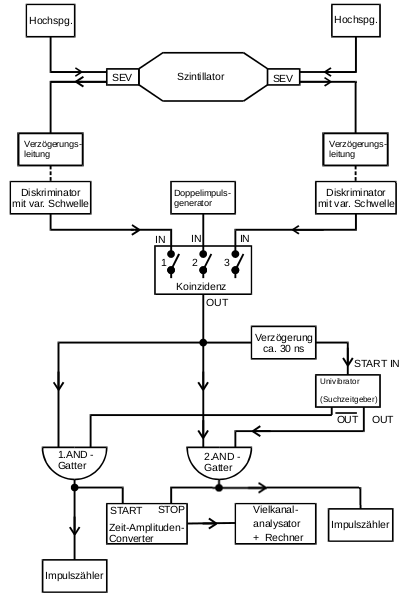
\includegraphics{Bilder/aufbau.png}
%	\label{fig:aufbau}
%\end{figure}
%
%\begin{figure}
%	\centering
%	\caption{Schematische Darstellung der Quelle zur Erzeugung radioaktiven Isotopen \cite{anleitung}.}
%	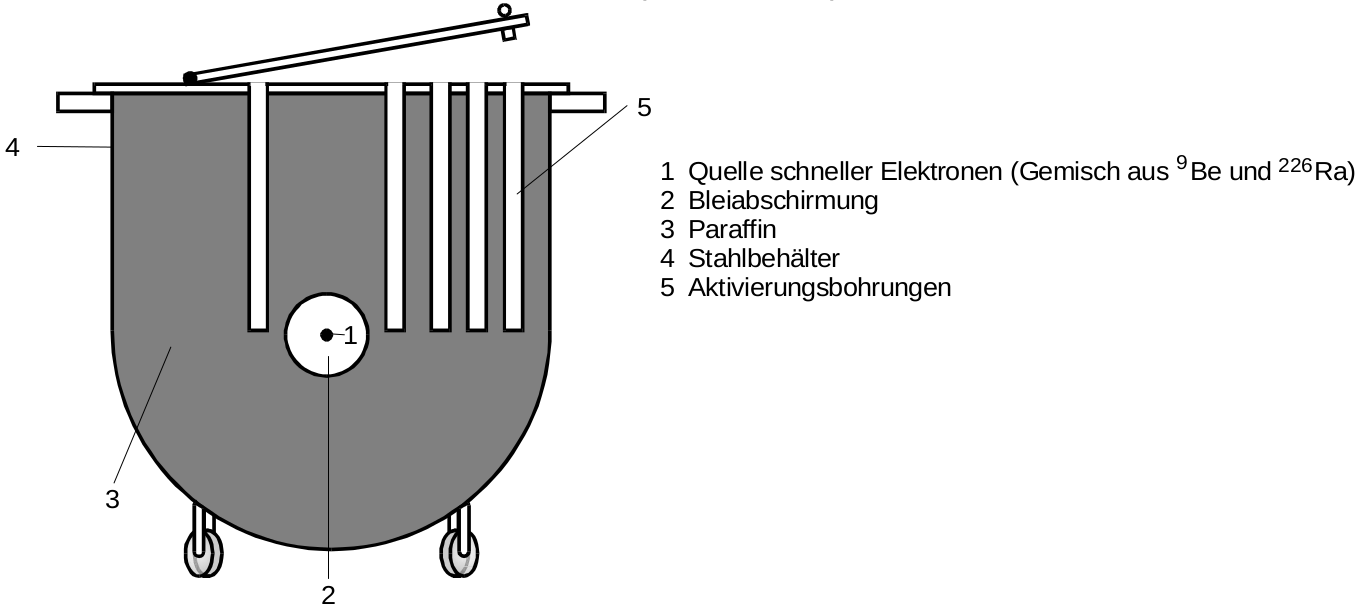
\includegraphics{content/toepfchen.png}
%	\label{fig:kochen}
%\end{figure}
%
Der Versuchsaufbau -- wie in Abbildung \ref{fig:aufbau} dargestellt -- besteht im Wesentlichen 
aus einem zerfallenden radioaktiven Isotop und einem Geiger-Müller-Zählrohr, welches die 
zerfallenden Kerne misst.
Das Geiger-Müller-Zählrohr ist entspricht einer mit Gas gefüllten Röhre. Trifft ein $\beta$-
oder $\gamma$- Teilchen auf ein Gasteilchen wird dieses ionisiert und kann aufgrund einer
anliegenden Spannung an der Röhre gemessen werden.
Dabei werden die gemessenen Zerfälle pro Messzeitintervall, welches am Zeitgeber einstellbar 
ist, an den Zählern 1 und 2 angezeigt. Nach jedem Messvorgang wird der Zähler umgeschaltet und 
der vorherige Wert auf dem aktuellen Zähler wird überschrieben. Der Versuchsaufbau ist mit
einer Blei-Abschirmung ausgestattet um die radioaktive Strahlung abzuschirmen.

Zur Erzeugung der radioaktiven Isotope wird das Objekt in Abbildung \ref{fig:kochen} verwendet.
Hierbei werden stabile Kerne mit niederenergetischen Neutronen beschossen. 
Da die Neutronen ihre Energie durch elastische Stöße an die Kerne übergeben und die maximale
Energie bei gleichen Massen der Stoßpartner erreicht wird, werden die Neutronen in einem 
Paraffinmantel gebremst, bis sie die optimale Energie besitzen.


\subsection{Versuchsbeschreibung}
\label{sec:Versuchsbeschreibung}
Zunächst wird der Acrylblock sowie die Fehlstellen mittels einer Schiebelehre vermessen.

Zur Bestimmung der Lage der Fehlstellen mit dem Impuls-Echo-Verfahren wird das Ultraschallechoskop über den Kippschalter auf den entsprechenden Messmodus (REFLEC.) gestellt.
Zunächst wird die tatsächlich auftretende Lauftzeit des Ultraschallsignals durch den Acrylblock bestimmt und mit dem theoretisch berechneten Wert verglichen, um die Dicke der Ausgleichsschit bestimmen zu können.
Die Ultraschallsonde mit \SI{1}{\mega\Hz} wird mittels bidestillierten Wasser an den Acrylblock gekoppelt, welcher auf eine weiche Unterlage gestellt wird, um eine Beschädigung des Acrylblocks zu vermeiden.
An verschiedenen Stellen des Acrylblocks wird über einen \textbf{A-Scan} die Schalllaufzeit zur Ermittlung der Lage der Störstellen gemessen. Selbige Prozedur wird wiederholt, nachdem der Block umgedreht wurde und die Ultraschallsonde von der anderen Seite an den Acrylblock gekoppelt wurde.
Zur Untersuchung des Auflösungsvermögens wird eine Impuls-Echo-Messung mit der $\SI{4}{\mega\Hz}$-Sonde für die zwei nach nebeneinander liegende Störstellen (Fehlstellen 1\&2 in Abbildung \ref{fig:stoerstellen}) durchgeführt und mit den Ergebnissen der Messung mit der $\SI{1}{\mega\Hz}$-Sonde verglichen.
Die Ultraschallsonde wird hierfür erneut mittels bidestillierten Wasser an den Acrylblock gekoppelt.

Die Bestimmung der Lage der Fehlstellen wird zudem über den \textbf{B-Scan} realisiert. Hierzu wird die $\SI{1}{\mega\Hz}$-Sonde mittels bidestillierten Wassers an den Probenblock gekoppelt, die Aufnahme des \textbf{B_Scan} gestartet, und der Acrylblock wird mit der Ultraschallsonde langsam abgefahren.
Ebenso wie beim \textbf{A-Scan} wird die Messung bei umgedrehten Block wiederholt.

Zur Untersuchung des Herzmodells wird dieses zu etwa einem Drittel mit bidestillierten Wasser gefüllt und die $\SI{1}{\mega\Hz}$-Sonde so auf der Wasseroberfläche positioniert, dass sie soeben eintaucht. Mittels eines Handblasebalg ist es möglich, die Gummimembran zu bewegen, sodass der Abstand zwischen der Ultraschallsonde und der Membran verringert wird. Hierbei muss die Verstärkung so gewählt werden, dass die Signale im \textbf{TM-Scan} deutlich zu sehen sind, zugleich aber auch nicht den Messbereich überschreiten.
Es wird ein \textbf{TM-Scan} mit $\SI{100}{\second}$ Laufzeit durchgeführt. Während der Messung wird der Handblasebalg möglichst gleichmäßig betätigt, um den Herzschlag zu simulieren.

\section{Auswertung}
\label{sec:Auswertung}
%***********************************************Auswertung a*************************
\subsection{Charakteristik des untersuchten Halogen-Zählrohrs}
Zur Untersuchung der Charakteristik des Halogen-Zählrohrs wird die gemessene Anzahl an Impulsen pro Minute auf Impulse pro Sekunde umgerechnet und gegen die angelegte Spannung aufgetragen.


\begin{longtable}{ccc}
  \caption{Messdaten zur Untersuchung der Charakteristik des Zählrohrs.}\label{tab:atab}\\
\toprule
$U$/$\si{\volt}$ &$N$/$\si{\minute}$&$N_\mathrm{sec}$/$\si{\second}$ \\

\midrule
\endhead
\midrule
\endfoot
450  & 0  & 0.0\\
460  & 35050  & \num{584.17(41)} \\
470  & 35724  & \num{595.40(41)} \\
480  & 36480  & \num{608.00(41)} \\
490  & 36574  & \num{609.57(41)} \\
500  & 36961  & \num{616.02(40)} \\
510  & 37141  & \num{619.02(40)} \\
520  & 36881  & \num{614.68(40)} \\
530  & 37379  & \num{622.98(40)} \\
540  & 37176  & \num{619.60(40)} \\
550  & 37276  & \num{621.27(40)} \\
560  & 37621  & \num{627.02(40)} \\
570  & 37201  & \num{620.02(40)} \\
580  & 37326  & \num{622.10(40)} \\
590  & 37541  & \num{625.68(40)} \\
600  & 37594  & \num{626.57(40)} \\
610  & 37640  & \num{627.33(40)} \\
620  & 37334  & \num{622.23(40)} \\
630  & 37986  & \num{633.10(40)} \\
640  & 38002  & \num{633.37(40)} \\
650  & 38058  & \num{634.30(40)} \\
660  & 37629  & \num{627.15(40)} \\
670  & 37353  & \num{622.55(40)} \\
680  & 37637  & \num{627.28(40)} \\
690  & 37815  & \num{630.25(40)} \\
700  & 37743  & \num{629.05(40)} \\
710  & 37716  & \num{628.60(40)} \\
720  & 37938  & \num{632.30(40)} \\
730  & 38047  & \num{634.12(40)} \\
740  & 38104  & \num{635.07(40)} \\
750  & 37755  & \num{629.25(40)} \\
760  & 37662  & \num{627.70(40)} \\
770  & 37877  & \num{631.28(40)} \\
780  & 38182  & \num{636.37(40)} \\
790  & 38128  & \num{635.47(40)} \\
800  & 38142  & \num{635.70(40)} \\
810  & 38252  & \num{637.53(40)} \\
820  & 37984  & \num{633.07(40)} \\
830  & 38063  & \num{634.38(40)} \\
840  & 38422  & \num{640.37(40)} \\
850  & 38423  & \num{640.38(40)} \\
860  & 38492  & \num{641.53(39)} \\
870  & 38650  & \num{644.17(39)} \\
880  & 38624  & \num{643.73(39)} \\
890  & 38462  & \num{641.03(39)} \\
900  & 38285  & \num{638.08(40)} \\
\bottomrule
\end{longtable}


In Tabelle \ref{tab:atab} finden sich die gemessenen Datentupel aus angelegter Spannung $U$ und gezählten Impulsen $N$ pro Minute. Zudem werden die hieraus berechneten Impulse pro Sekunde $N_\mathrm{sec}$ und die Breite des zugehörigen Vertrauensintervall $\frac{\sqrt{N_\mathrm{sec}}}{N_\mathrm{sec}}$ angegeben.\\
In Abbildung \ref{fig:a} findet sich die Zählrohrcharakteristik.
Da der Bereich der Dauerentladung mit der vorliegenden Messapparatur nicht erreicht wurde, und die Anzahl der gemessenen Impulse zum Ende der Messung wieder leicht sinkt, wird ein Fehler im Versuch vermutet und als Arbeitsbereich des Zählrohrs das Intervall von $\SI{480}{\volt}$ bis $\SI{870}{\volt}$ angenommen.
Es ergibt sich somit eine Plateaulänge von $\Delta U_\mathrm{P}=\SI{390}{\volt}$.
Im Arbeitsbereich des Zählrohrs wird eine lineare Ausgleichsrechnung mit python/scipy \cite{scipy} durchgeführt.\\
Es ergeben sich die Parameter der Ausgleichgraden $y=m\cdot x+b$ zu:
\begin{align}
  m=  \SI{0.061(5)}{\volt\per\second} \text{,}\\
  b=  \SI{587(4)}{\per\second}\text{.}
\end{align}

Aus der Steigung der Ausgleichsgraden lässt sich die Steigung $P_\mathrm{S}$ im Plateaubereich ablesen zu:
\begin{equation*}
  P_\mathrm{S}=\frac{\SI{6.1(5)}{\percent}}{\SI{100}{\volt}} \text{ .}
\end{equation*}
\begin{figure}
  \centering
  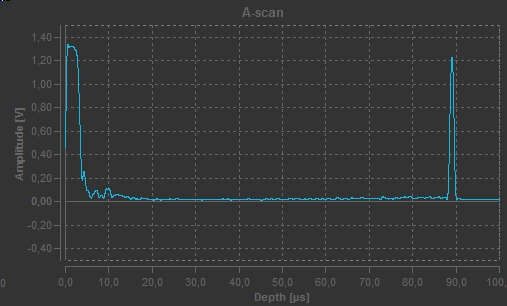
\includegraphics{Bilder/a.pdf}
  \caption{Zählrohrcharakteristik des Halogen-Zählrohrs samt markierter Plateaulänge und Ausgleichsgraden zur Bestimmung der Plateausteigung.}
  \label{fig:a}
\end{figure}
\FloatBarrier
%***********************************************

\subsection{Untersuchung von Nachentladungen}
Der Vergleich des Oszilloskopbilds bei einer geringen Betriebsspannung von etwa $\SI{450}{\volt}$ mit einer hohen Betriebsspannung von etwa $\SI{700}{\volt}$ zeigt, dass häufige und deutliche Nachentladungen lediglich für hohe Betriebsspannungen am Oszilloskopschirm sichtbar werden.
Nach Abbildung \ref{fig:nachladen} wird die Zeit zwischen dem ersten Impuls und den Nachentladungen abgelesen zu $\Delta t=\SI{175}{\micro\second}$.


\subsection{Bestimmung der Totzeit aus dem Oszilloskopbild}
Die Totzeit lässt sich nach Abbildung \ref{fig:nachladen} aus dem Oszilloskop ablesen.
In Tabelle \ref{tab:c} finden sich die bei verschiedenen Betriebsspannungen abgelesenen Totzeiten $T$, sowie die zugehörigen Erholungszeiten $T_\mathrm{E}$.
Da diese sich sehr willkürlich und nur ungenau bestimmen lassen, ist eine weitere Betrachtung der Erholungszeiten nicht sinnvoll.
\begin{table}
  \centering
  \caption{Messdaten zur Bestimmung der Totzeit aus dem Oszilloskopbild.}
  \label{tab:c}
\begin{tabular}{ccc}
  \toprule
$U$/$\si{\volt}$ & $T$/$\si{\micro\second}$ & $T_\mathrm{E}$/$\si{\micro\second}$ \\
\midrule
450  & 175  & 150  \\
500  & 175  & 100  \\
550  & 175  & 125  \\
600  & 175  & 150  \\
650  & 175  & 200  \\
\bottomrule
\end{tabular}
\end{table}
Eine Mittelung über alle Totzeiten ergibt eine mittlere Totzeit von $\overline{T}=\SI{175}{\micro\second}$.

\subsection{Bestimmung der Totzeit über die Zwei-Quellen-Methode}
\begin{table}
  \centering
  \caption{Messdaten zur Bestimmung der Totzeit über die Zwei-Quellen-Methode.}
  \label{tab:tot}
\begin{tabular}{ccc}
  \toprule
Quelle& $N$/$\si{\minute}$& $N$/$\si{\second}$ \\
\midrule
$N_1$ & 3499 & \num{58.3(1)} \\
$N_{1+2}$ & 49676 & \num{827.93(4)} \\
$N_{2}$ & 46298 & \num{771.63(4)} \\
\bottomrule
\end{tabular}
\end{table}
In Tabelle \ref{tab:tot} finden sich die gemessenen Impulsraten der Messung zur Bestimmung der Totzeit über die Zwei-Quellen-Methode.
Es wird erneut nach der Poisson-Verteilung ein Vertrauensintervall von $\pm\frac{\sqrt{N_i}}{N_i}$ angenommen.
Nach Formel \eqref{eqn:totzeit} ergibt sich die Totzeit zu:
\begin{equation}
  T=\SI{22.4(2)}{\micro\second}
\end{equation}

%Bild
%\begin{figure}
%  \centering
%  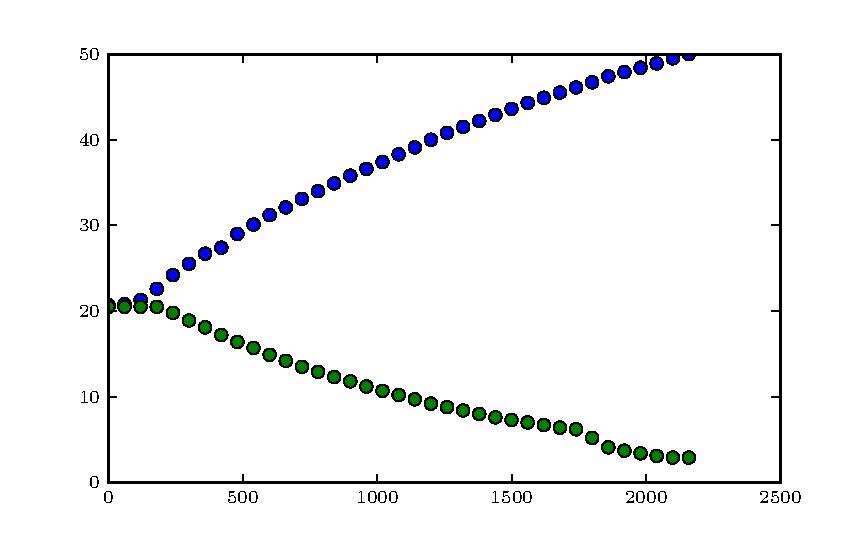
\includegraphics{plot.pdf}
%  \caption{Plot.}
%  \label{fig:plot}
%\end{figure}


%Tabelle
%\begin{table}
%	\centering
%	\caption{Table.}
%	\label{tab:table}
%	\begin{tabular}{ccc}
%		\toprule
%    column1&column2&column3\\
%		\midrule
%		220 & -391 & 659 \\
%		330 & -598 & 946 \\
%		525 & -1000 & 1660 \\
%		702 & -1337 & 2051 \\
%		930 & -1650 & 2450 \\
%		\bottomrule
%	\end{tabular}
%\end{table}

\section{Diskussion}
\label{sec:Diskussion}
Das Experiment ist äußerst empfindlich für äußere Einflüsse. Leichte Bewegungen oder Positionsänderungen in der Nähe des Experiments verursachten große Schwankungen im Oszilloskopbild.\\
Es könnten daher prinzipiell unbemerkte systematische Fehler aufgetreten sein.

Da das Amplitudenverhältnis nur aus einem abfotografierten Oszilloskopbild bestimmt wurde und der Wert maximaler Transparenz nicht ganz eindeutig bestimmbar ist, sind besonders hier Ablesefehler nicht auszuschließen.\\
In der Dampfkammer lag ein Isotopenverhältnis von $\frac{A_1}{A_2}=\frac{\ce{^87Rb}}{\ce{^85Rb}}\approx 0.58\pm 0.02$ vor. Natürlich kommt ein Verhältnis von $\frac{\ce{^87Rb}}{\ce{^85Rb}}\approx 0.39$ vor \cite{muenster}.\\
Nach unserer Messung ist also die Konzentration von $\ce{^87Rb}$ deutlich höher, als seine Konzentration im natürlichen Vorkommen.\\
Die vorliegende Messung zeigt eine Abweichung von etwa $33\%$ im Verhältnis der Rubidium-Isotope im Vergleich zum natürlichen Vorkommen.\\
Wie bereits erwähnt, könnte das bestimmte Amplitudenverhältnis allerdings aufgrund von Ablesefehlern ungenau sein.

In Tabelle \ref{tab:discuss} findet sich ein Vergleich der experimentell bestimmten Werte mit den Theoriewerten.\\
Die größte Abweichung zeigt sich in der Bestimmung der Vertikalkomponente des Erdmagnetfelds. Der experimentelle Wert errechnete sich lediglich über einen Messwert, ein Fehler hierbei würde sich also direkt deutlich auswirken.\\
Alle anderen experimentellen Werte liegen allerdings sehr nah an den Theoriewerten, besonders in der Messung der Kernspins und der Landéschen Faktoren (Abweichungen $<1\%$) scheint also kein systematischer Fehler vorliegen zu können.\\
\begin{table}
  \caption{Vergleich der bestimmten Größen mit den Literaturwerten}
  \label{tab:discuss}
 \centering
 \begin{tabular}{cccc}
   \toprule
Messgröße&Experiment&Theorie&prozentuale Abweichung\\
\midrule
Erdmagnetfeld, vertikal&$\SI{35400}{\nano\tesla}$&$\SI{45012.9}{\nano\tesla}$&$21.3\%$\\
Erdmagnetfeld, horizontal&$\SI{18.3(5)e-6}{\tesla}$&$\SI{19304.4}{\nano\tesla}$&$5.2\%$\\
Kernspin $I$ $\ce{^87Rb}$&$1.491\pm0.021$&$\frac{3}{2}$&$0.5\%$\\
$g_{\mathrm{F}}$ von $\ce{^87Rb}$&$0.503\pm0.005$&$\frac{1}{2}$&$0.6\%$\\
Kernspin $I$ $\ce{^85Rb}$&$2.515\pm0.009$&$\frac{5}{2}$&$0.6\%$\\
$g_{\mathrm{F}}$ von $\ce{^85Rb}$&$0.332\pm0.001$&$\frac{1}{3}$&$0.4\%$\\
\bottomrule
\end{tabular}
\end{table}
Die Theoriedaten der Magnetfeldstärken des Erdmagnetfelds wurden hierbei mit dem Deklinationsrechner des GFZ Potsdam für Dortmund ermittelt \cite{dekli}.
Die Theoriewerte der Kernspins ergeben sich nach \cite{muenster}, die Theoriewerte der Landéschen Faktoren nach \cite{gf} für $\ce{^87Rb}$ und \cite{gf2} für $\ce{^85Rb}$.

%input{content/datenanhang.tex}

\printbibliography

\end{document}
